%%%
%%% za primere: set_display(none)$ linel:60$.
%%%

\documentclass[11pt]{article}

\usepackage[a4paper]{geometry}
\usepackage{graphicx}
\usepackage{fancyvrb}

\usepackage{hyperref}

\usepackage{mathpazo}
\linespread{1.05}

\usepackage{tikz}
\usetikzlibrary{decorations.pathmorphing}
\tikzstyle{every node}=[fill=white,draw=black,shape=circle,inner sep=1mm]

\newcommand{\command}[1]{\texttt{#1}}
\newcommand{\maxima}{\textsc{Maxima}}
\newcommand{\species}[1]{\mathcal{#1}}
\newcommand{\DEF}[1]{{\em #1}}
\newcommand{\LINK}[1]{\href{#1}{#1}}

\newtheorem{theorem}{Theorem}

\DefineVerbatimEnvironment{example}{Verbatim}{%
	frame=leftline,%
	rulecolor=\color{gray},%
	framerule=2pt,%
	framesep=3mm}

\begin{document}

\title{Counting with generating functions in \maxima}
\author{Andrej Vodopivec\\ \texttt{andrej.vodopivec@gmail.com}}
\date{}
\maketitle

\abstract{An implementation of packages for P\'olya theory and
combinatorial species for the computer algebra system
\maxima\ is presented.}

%%%%%%%%%%%%%%%%%%%%%%%%%%%%%%%%%%%%%%%%%%%%%%%%%%
%%%%%%%%%%%%%%%%%%%%%%%%%%%%%%%%%%%%%%%%%%%%%%%%%%
%%%%%%%%%%%%%%%%%%%%%%%%%%%%%%%%%%%%%%%%%%%%%%%%%%
\section{Introduction}

A large part of combinatorics is concerned with counting. Many
counting problems can be efficiently solved by using generating
functions. In this paper we describe implementations of two counting
methods which are based on generating functions for the computer
algebra system \maxima\cite{Max}.

P\'olya theory \cite{P} is an important counting method when some
objects that are being counted have to be considered equal because of
symmetry. The package \command{discrete} provides basic functionality
for working with permutation groups and applications of P\'olya's
theorems. The package also adds some extensions to the maxima
\command{graphs} package and defines functions for other topics in
discrete mathematics, but this functionality will not be described in
this paper.

The package \command{Species} implements methods for working with
combinatorial spe\-cies \cite{J,BLL}. The theory of combinatorial
species can be applied when we are counting objects which are built
from smaller objects using some production rules. The most well known
package for combinatorial species is the \command{combstruct} package
for Maple. Open--source implementations include MuPAD-Combinat
\cite{MCS}, \cite{MC}, Aldor-Combinat \cite{AC} and the species
package of Sage \cite{sage}. The package \command{Species} described
in this paper currently only implements unlabelled species only and
provides functions for counting, listing and random generation of
combinatorial species.

The paper is divided into two parts. The first describes P\'olya
theory and the second combinatorial species. Both parts start with
short theoretical background and then expose the packages with worked
examples in \maxima. The packages require \maxima\ version 5.22 or
above.

%%%%%%%%%%%%%%%%%%%%%%%%%%%%%%%%%%%%%%%%%%%%%%%%%%
%%%%%%%%%%%%%%%%%%%%%%%%%%%%%%%%%%%%%%%%%%%%%%%%%%
%%%%%%%%%%%%%%%%%%%%%%%%%%%%%%%%%%%%%%%%%%%%%%%%%%
\section{P\'olya theory}

%%%%%%%%%%%%%%%%%%%%%%%%%%%%%%%%%%%%%%%%%%%%%%%%%%
%%%%%%%%%%%%%%%%%%%%%%%%%%%%%%%%%%%%%%%%%%%%%%%%%%
\subsection{Permutation groups}

The package \command{discrete} provides several functions for working
with permutations. Some basic group theory functions are also
present. The purpose is applications in P\'olya theory.

The function \command{permutation\_product} computes a product of
permutations. By default the product is from left to right.  The order
can be specified with the option variable
\command{permutation\_multiplication} (valid values are
\command{left\_to\_right} and \command{right\_to\_left}. A permutation
power can be efficiently computed with the function
\command{permutation\_power}.

The function \command{permutation\_to\_cycles} transforms a
permutation to the product of disjoint cycles. The reverse can be done
with \command{permutation\_from\_cycles}. There are similar functions
for converting a permutation to a product of transpositions and back.

\begin{example}
(%i1) load(discrete)$
(%i2) a: random_permutation([1,2,3,4,5,6,7,8]);
(%o2) [2,5,8,3,7,4,1,6]
(%i3) permutation_to_cycles(%);
(%o3) [[1,2,5,7],[3,8,6,4]]
(%i4) permutation_from_cycles([[1,2,3,4], [5,6]], 10);
(%o4) [2,3,4,1,6,5,7,8,9,10]
(%i5) permutation_power(a, 10);
(%o5) [5,7,6,8,1,3,2,4]
\end{example}
%
A permutation group is represented as a set of permutation. It can be
generated from a set of generators with the function
\command{group\_from\_generators} (some functions accept a set of
generators instead of the whole group and an optional argument
\command{generators=true}).

\begin{example}
(%i6) group_from_generators({[2,3,4,5,1], [1,5,4,3,2]});
(%o6) {[1,2,3,4,5],[1,5,4,3,2],[2,1,5,4,3],[2,3,4,5,1],
       [3,2,1,5,4],[3,4,5,1,2],[4,3,2,1,5],[4,5,1,2,3],
       [5,1,2,3,4],[5,4,3,2,1]}
\end{example}
%
An important class of problems deal with groups of automorphisms of
graphs. The package \command{discrete} provides a function
\command{graph\_automorphisms} which can generate the group of
automorphisms of the graph or only the generators of the group.
%
\begin{example}
(%i7) g:grid_graph(3,7)$
(%i8) graph_automorphisms(g);
(%o8) {[1,2,3,4,5,6,7,8,9,10,11,12,13,14,15,16,17,18,19,20,21],
       [3,2,1,6,5,4,9,8,7,12,11,10,15,14,13,18,17,16,21,20,19],
       [19,20,21,16,17,18,13,14,15,10,11,12,7,8,9,4,5,6,1,2,3],
       [21,20,19,18,17,16,15,14,13,12,11,10,9,8,7,6,5,4,3,2,1]}
\end{example}
%
For larger graphs an external program called \command{bliss}
\cite{bliss} can be used to find the automorphisms.  The
\command{bliss} program must be installed separately and the path to
the program must be specified in the variable
\command{bliss\_program}.
%
\begin{example}
(%i9) bt4: binary_tree(4)$
(%i10) gens: graph_automorphisms(bt4,program=bliss,generators=true)$
(%i11) group_order(gens);
(%o11) 32768
(%i12) group_orbits(gens, generators=true);
(%o12) {{1,2,4,5,8,9,11,12,16,17,19,20,23,24,26,27},
        {3,6,10,13,18,21,25,28},{7,14,22,29},{15,30},{31}}
\end{example}

%%%%%%%%%%%%%%%%%%%%%%%%%%%%%%%%%%%%%%%%%%%%%%%%%%
%%%%%%%%%%%%%%%%%%%%%%%%%%%%%%%%%%%%%%%%%%%%%%%%%%
\subsection{P\'olya theory}

A \DEF{cycle index} of a permutation $\pi$ is the monomial $Z(\pi;
x_1, \ldots, x_k)=x_1^{n_1}x_2^{n_2}\cdots x_k^{n_k}$ where $n_i$ is
the number of cycles of length $i$ in the representation of $\pi$ as
the product of disjoint cycles.

\begin{example}
(%i1) load(discrete)$
(%i2) pi: random_permutation(int_range(10));
(%o2) [4,9,8,3,5,10,7,1,2,6]
(%i3) permutation_to_cycles(pi);
(%o3) [[1,4,3,8],[2,9],[6,10]]
(%i4) cycle_index_permutation(pi);
(%o4) x[1]^2*x[2]^2*x[4]
\end{example} 
%
The cycle index of a permutation group $G$ is the average of cycle
indexes of permutations in $G$:
$$
Z(G;x_1,\ldots,x_k) = \frac{1}{|G|}\sum_{\pi\in G}Z(\pi; x_1,\ldots,x_k).
$$
There are many functions to compute the cycle index of groups.
\begin{example}
(%i5) s4: symmetric_group(4)$
(%i6) cycle_index_group(s4);
(%o6) (6*x[4]+8*x[1]*x[3]+3*x[2]^2+6*x[1]^2*x[2]+x[1]^4)/24
(%i7) cycle_index_symmetric(4);
(%o7) (6*x[4]+8*x[1]*x[3]+3*x[2]^2+6*x[1]^2*x[2]+x[1]^4)/24
(%i8) cycle_index_dihedral(7);
(%o8) (6*x[7]+x[1]^7)/14+(x[1]*x[2]^3)/2
\end{example}
%
Let $X$ and $Y$ be finite sets and $\mathcal{F}=\{f:X\to Y\}$ the set
of mappings from $X$ to $Y$. Let $G$ be a group acting on $X$. We
define an equivalence relation $\sim_G$ on $\mathcal{F}$ as
$$
f_1 \sim_G f_2 \quad \Longleftrightarrow \quad
\mbox{$\exists g\in G\ \forall x\in X: \ f_1(x)=f_2(x^g)$.}
$$
We say that $f_1$ and $f_2$ differ by the symmetry $g$. We are
interested in the number of equivalence classes of the relation
$\sim_G$. The equivalence classes are called \DEF{patterns}.

\begin{theorem}
\label{thm:polya1}
If the size of the set $Y$ is $|Y|=r$ then the number of equivalence
classes in the relation $\sim_G$ is
$$
Z(G; r,\ldots, r).
$$
\end{theorem}
The can be applied with the \command{subst\_inventory(r, ci)} command.

Suppose further we have a set $W$ of weights and a weight function
$w:Y\to W$. For a pattern $C$ and $f\in C$ we define a \DEF{pattern
  inventory of $C$} as
$$
PI(C) = \prod_{x\in X} w(f(x)).
$$
Note that the choice of $f$ is not important.

A \DEF{pattern inventory of the group $G$} is then defined as
$$
PI(G) = \sum_{n_1+\cdots+n_k=n}\tau(n_1,\ldots, n_k)[w(y_i)]^{n_1}\cdots [w(y_k)]^{n_k}.
$$
where $\tau(n_1,\ldots,n_k)$ is the number of patterns with the
pattern inventory
$$
[w(y_i)]^{n_1}\cdots [w(y_k)]^{n_k}.
$$

\begin{theorem}
\label{thm:polya2}
Let $s_i=[w(y_1)]^i+\cdots+[w(y_r)]^i$. Then
$$
PI(G) = Z(G; s_1,\ldots, s_k).
$$
\end{theorem}
The theorem can be applied with the
\command{subst\_inventory([w(y1),\ldots,w(yk)], ci)} command.

%%%%%%%%%%%%%%%%%%%%%%%%%%%%%%%%%%%%%%%%%%%%%%%%%%
%%%%%%%%%%%%%%%%%%%%%%%%%%%%%%%%%%%%%%%%%%%%%%%%%%
\subsection{Examples}

%%%%%%%%%%%%%%%%%%%%%%%%%%%%%%%%%%%%%%%%%%%%%%%%%%
\subsubsection{Necklaces and bracelets}

A $n$-airy necklace of is composed of $n$ colored beads arranged in a
circle. Two necklaces are the same if we can rotate the first necklace
so that the colors of the beads match the colors of the second
necklace.

\begin{figure}
\begin{center}
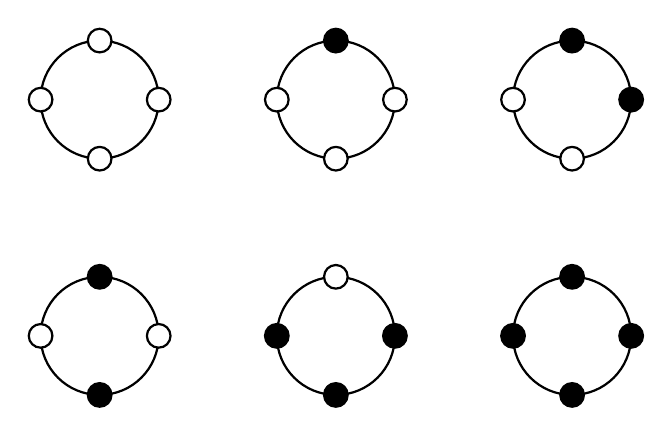
\begin{tikzpicture}[style=thick, scale=1.5]
	\draw (0.5,2.5) circle (0.5cm);
		\draw[fill=white]
			(0.5,2) circle (1mm)
			(0,2.5) circle (1mm)
			(1,2.5) circle (1mm)
			(0.5,3) circle (1mm);
	\draw (2.5,2.5) circle (0.5cm);
		\draw[fill=white]
			(2,2.5) circle (1mm)
			(3,2.5) circle (1mm)
			(2.5,2) circle (1mm);
		\draw[fill=black]
			(2.5,3) circle (1mm);
	\draw (4.5,2.5) circle (0.5cm);
		\draw[fill=white]
			(4.5,2) circle (1mm)
			(4,2.5) circle (1mm);
		\draw[fill=black]
			(4.5,3) circle (1mm)
			(5,2.5) circle (1mm);
	\draw (0.5,0.5) circle (0.5cm);
		\draw[fill=black]
			(0.5,0) circle (1mm)
			(0.5,1) circle (1mm);
		\draw[fill=white]
			(1,0.5) circle (1mm)
			(0,0.5) circle (1mm);
	\draw (2.5,0.5) circle (0.5cm);
		\draw[fill=white]
			(2.5,1) circle (1mm);
		\draw[fill=black]
			(3,0.5) circle (1mm)
			(2.5,0) circle (1mm)
			(2,0.5) circle (1mm);
	\draw (4.5,0.5) circle (0.5cm);
		\draw[fill=black]
			(4.5,1) circle (1mm)
			(5,0.5) circle (1mm)
			(4.5,0) circle (1mm)
			(4,0.5) circle (1mm);
\end{tikzpicture}
\end{center}
\caption{4--airy necklaces of with 2 colors.}
\label{fig:necklaces2}
\end{figure}

Let $X$ be the set of $n$ beads arranged on a circle and $Y$ the set
of colors. A $n$-airy necklace is a mapping $f:X\to Y$ which assigns
the color $f(x)$ to each bead $x\in X$. Let $G$ be a cyclic group of
order $n$ acting on the set $X$. Two necklaces $f_1$ and $f_2$ are the
same if there is an element $g\in G$ such that $f_2(x)=f_1(x^g)$ for
all beads $x\in X$. In order to count the number of $n$-airy necklaces
we apply Theorem \ref{thm:polya1}. If we we need to substitute $r=|Y|$
into the cycle index of the group $G$ we obtain the number of $n$-airy
necklaces.

The number of 4-airy necklaces colored with two or four colors can be
computed in \maxima\ as follows.

\begin{example}
(%i1) load(discrete)$
(%i2) ci: cycle_index_cyclic(4);
(%o2) (2*x[4]+x[2]^2+x[1]^4)/4
(%i3) subst_inventory(2, ci);
(%o3) 6
(%i4) subst_inventory(4, ci);
(%o4) 70
\end{example}
%
The necklaces with colors white and black are shown in Figure
\ref{fig:necklaces2}. Using the Theorem \ref{thm:polya2} we can
further divide the numbers according to how many beads are colored
with the color black. We assign weight 1 to the color white and weight
$b$ to the color black. The coefficient at $b^m$ tells us the number
of necklaces with $m$ beads colored with the color black.

\begin{example}
(%i5) subst_inventory([1,b], ci);
(%o5) b^4+b^3+2*b^2+b+1
\end{example}
%
If we are interested in necklaces with four colors in which colors red
and green both appear exactly once, we assign the weights $r$ and $g$
to colors red and green and the weights 1 to the other two colors.

When we substitute the inventory into the cycle index we obtain the
pattern inventory, from which we need to read the coefficient at the
monomial $r g$.

\begin{example}
(%i6) inv: subst_inventory([r,g,1,1], ci);
(%o6) r^4+g*r^3+2*r^3+2*g^2*r^2+6*g*r^2+7*r^2+g^3*r
         +6*g^2*r+12*g*r+8*r+g^4+2*g^3+7*g^2+8*g+6
(%i7) mcoeff(inv,r,1,g,1);
(%o7) 12
\end{example}
%
If we replace the cyclic group with the dihedral group we also do not
distinguish between necklaces if they differ by a reflection.  Such
necklaces are called bracelets.

\begin{figure}[t]
\begin{center}
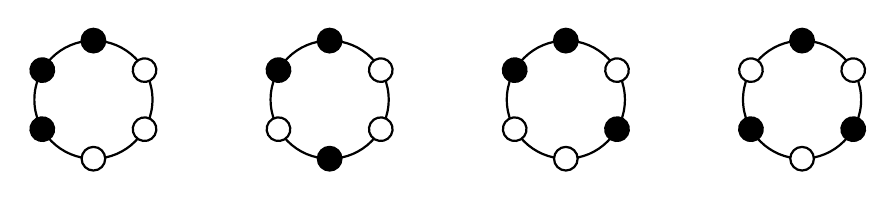
\begin{tikzpicture}[style=thick, scale=1.5]
\draw (0.5, 0.5) circle (0.5cm);
	\draw[fill=black] (0.5,1) circle (1mm);
	\draw[fill=black, rotate around={60:(0.5, 0.5)}] (0.5,1) circle (1mm);
	\draw[fill=black, rotate around={120:(0.5, 0.5)}] (0.5,1) circle (1mm);
	\draw[fill=white, rotate around={180:(0.5, 0.5)}] (0.5,1) circle (1mm);
	\draw[fill=white, rotate around={240:(0.5, 0.5)}] (0.5,1) circle (1mm);
	\draw[fill=white, rotate around={300:(0.5, 0.5)}] (0.5,1) circle (1mm);
\draw (2.5, 0.5) circle (0.5cm);
	\draw[fill=black] (2.5,1) circle (1mm);
	\draw[fill=black, rotate around={60:(2.5, 0.5)}] (2.5,1) circle (1mm);
	\draw[fill=white, rotate around={120:(2.5, 0.5)}] (2.5,1) circle (1mm);
	\draw[fill=black, rotate around={180:(2.5, 0.5)}] (2.5,1) circle (1mm);
	\draw[fill=white, rotate around={240:(2.5, 0.5)}] (2.5,1) circle (1mm);
	\draw[fill=white, rotate around={300:(2.5, 0.5)}] (2.5,1) circle (1mm);
\draw (4.5, 0.5) circle (0.5cm);
	\draw[fill=black] (4.5,1) circle (1mm);
	\draw[fill=black, rotate around={60:(4.5, 0.5)}] (4.5,1) circle (1mm);
	\draw[fill=white, rotate around={120:(4.5, 0.5)}] (4.5,1) circle (1mm);
	\draw[fill=white, rotate around={180:(4.5, 0.5)}] (4.5,1) circle (1mm);
	\draw[fill=black, rotate around={240:(4.5, 0.5)}] (4.5,1) circle (1mm);
	\draw[fill=white, rotate around={300:(4.5, 0.5)}] (4.5,1) circle (1mm);
\draw (6.5, 0.5) circle (0.5cm);
	\draw[fill=black] (6.5,1) circle (1mm);
	\draw[fill=white, rotate around={60:(6.5, 0.5)}] (6.5,1) circle (1mm);
	\draw[fill=black, rotate around={120:(6.5, 0.5)}] (6.5,1) circle (1mm);
	\draw[fill=white, rotate around={180:(6.5, 0.5)}] (6.5,1) circle (1mm);
	\draw[fill=black, rotate around={240:(6.5, 0.5)}] (6.5,1) circle (1mm);
	\draw[fill=white, rotate around={300:(6.5, 0.5)}] (6.5,1) circle (1mm);
\end{tikzpicture}
\end{center}
\caption{6-airy necklaces colored with three black and three white beads.}
\label{fig:necklaces6}
\end{figure}

We count the necklaces and bracelets of size 6 with three beads
colored black and three beads colored white.
\begin{example}
(%i8) ci: cycle_index_cyclic(6);
(%o8) (2*x[6]+2*x[3]^2+x[2]^3+x[1]^6)/6
(%i9) subst_inventory([1,t], ci);
(%o9) t^6+t^5+3*t^4+4*t^3+3*t^2+t+1
(%i10) coeff(%, t, 3);
(%o10) 4
(%i11) ci: cycle_index_dihedral(6);
(%o11) (2*x[6]+2*x[3]^2+x[2]^3+x[1]^6)/12+(x[2]^3+x[1]^2*x[2]^2)/4
(%i12) subst_inventory([1,t], ci);
(%o12) t^6+t^5+3*t^4+3*t^3+3*t^2+t+1
(%i13) coeff(%, t, 3);
(%o14) 3
\end{example}
%
6-airy necklaces with three black and three white beads are shown in
Figure \ref{fig:necklaces6}. The second and third necklace represent
the same bracelet.

In the last example we show how to obtain the list of 4--airy necklaces
with 2 colors using the \command{group\_orbits} function. We need to
define a set of all colorings of the 4--cycle (represented as a list),
and compute orbit representatives for the group action on the set of
colorings.

The possible colorings are binary sequences of length 4 and are
computed with the \command{bin\_seqs} function. We define the function
\command{permute\_list} which defines the action of the group on the
colorings. Finally we compute the group orbit representatives with the
\command{group\_orbit\_representatives} function. We need to specify
the set on which the group acts and the group action. We also only
wish to see representatives for each orbit. The result should be
compared with Figure \ref{fig:necklaces2}.

\begin{example}
(%i15) bin_seqs(n) :=
         if n=1 then [[1],[0]]
         else block([bs: bin_seqs(n-1)],
           append(
             map(lambda([s], cons(1, s)), bs),
             map(lambda([s], cons(0, s)), bs)))$
(%i16) grp: cyclic_group(4)$
(%i17) group_orbit_representatives(grp,
          set=setify(bin_seqs(4)), action=permute_list);
(%o17) {[0,0,0,0],[0,0,0,1],[0,0,1,1],[0,1,0,1],[0,1,1,1],
        [1,1,1,1]}
(%i18) length(%);
(%o18) 6
\end{example}

%%%%%%%%%%%%%%%%%%%%%%%%%%%%%%%%%%%%%%%%%%%%%%%%%%
\subsubsection{Colorings of graphs}

An important application of P\'olya theory is to molecular graphs
(graphs which represent molecules). An example of such graph
is shown in Figure \ref{fig:mgraph}.

\begin{figure}
\begin{center}
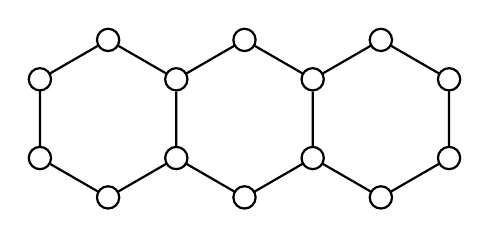
\begin{tikzpicture}[style=thick, scale=0.5]
	\draw (0,0) node (n1)  {} --
		 ++(90:2) node (n2) [] {} --
		 ++(30:2) node (n3) [] {} --
		 ++(-30:2) node (n4) [] {} --
		 ++(30:2) node (n5) [] {} --
		 ++(-30:2) node (n6) [] {} --
		 ++(30:2) node (n7) [] {} --
		 ++(-30:2) node (n8) [] {} --
		 ++(-90:2) node (n9) [] {} --
		 ++(-150:2) node (n10) [] {} --
		 ++(-210:2) node (n11) [] {} --
		 ++(-150:2) node (n12) [] {} --
		 ++(-210:2) node (n13) [] {} --
		 ++(-150:2) node (n14) [] {} -- (n1)
		(n4) -- (n13) (n6) -- (n11);
\end{tikzpicture}
\end{center}
\caption{A molecular graph.}
\label{fig:mgraph}
\end{figure}

In the next example we count 2--colorings of the graph in
Figure \ref{fig:mgraph} if we consider two colorings to be equal when
they differ by an automoprhism of the graph. We also count the number
of 2-colorings in which the first color appears twice. The package
\command{discrete} loads the \command{graphs} package so we can use
its functions to define the graph. We need to work around a technical
issue first. The graphs created with the \command{graphs} package have
vertex ids from 0 to $n-1$. We first relabel the vertices so that the
ids are from 1 to $n$.

\begin{example}
(%i1) load(discrete)$
(%i2) g: cycle_graph(14)$
(%i3) g: relabel_graph_vertices(g, min_id=1)$
(%i4) add_edges([[3,12],[5,10]], g)$
(%i5) grp: graph_automorphisms(g);
(%o5) {[1,2,3,4,5,6,7,8,9,10,11,12,13,14],
       [7,6,5,4,3,2,1,14,13,12,11,10,9,8],
       [8,9,10,11,12,13,14,1,2,3,4,5,6,7],
       [14,13,12,11,10,9,8,7,6,5,4,3,2,1]}
(%i6) ci: cycle_index_group(grp);
(%o6) (2*x[2]^7+x[1]^2*x[2]^6+x[1]^14)/4
(%i7) subst_inventory(2, ci);
(%o7) 4224
(%i8) inv: subst_inventory([1,t], ci);
(%o8) t^14+4*t^13+28*t^12+94*t^11+266*t^10+508*t^9+777*t^8
          +868*t^7+777*t^6+508*t^5+266*t^4+94*t^3+28*t^2
          +4*t+1
(%i9) coeff(inv, t, 2);
(%o9) 28
\end{example}
%
If we wish to count the number of 2--colorings of the edges of the graph,
we need to compute the group action of \command{grp} on the set 
edges of the graph.

\begin{example}
(%i10) edges: fullsetify(edges(g))$
(%i11) grp_e: group_action(grp, edges);
(%o11) {[1,2,3,4,5,6,7,8,9,10,11,12,13,14,15,16],
        [9,10,7,6,8,4,3,5,1,2,16,15,14,13,12,11],
        [11,10,12,13,8,14,15,5,16,2,1,3,4,6,7,9],
        [16,2,15,14,5,13,12,8,11,10,9,7,6,4,3,1]}
(%i12) ci_e: cycle_index_group(grp_e);
(%o12) (2*x[2]^8+x[1]^4*x[2]^6+x[1]^16)/4
(%i13) subst_inventory([1,t], ci_e);
(%o13) t^16+5*t^15+37*t^14+147*t^13+482*t^12+1113*t^11
           +2059*t^10+2895*t^9+3290*t^8+2895*t^7+2059*t^6
           +1113*t^5+482*t^4+147*t^3+37*t^2+5*t+1
\end{example}

%%%%%%%%%%%%%%%%%%%%%%%%%%%%%%%%%%%%%%%%%%%%%%%%%%
\subsubsection{Graphs generating function}

The \DEF{graph generating function} is defined as
$$
GF_n(t) = \sum_{m=0}^{\frac{n(n+1)}{2}} a_mt^m
$$
where $a_n$ is the number of graphs on $n$ vertices with $m$ edges.
In this example we compute the function $GF_4(t)$.

\begin{figure}
\begin{center}
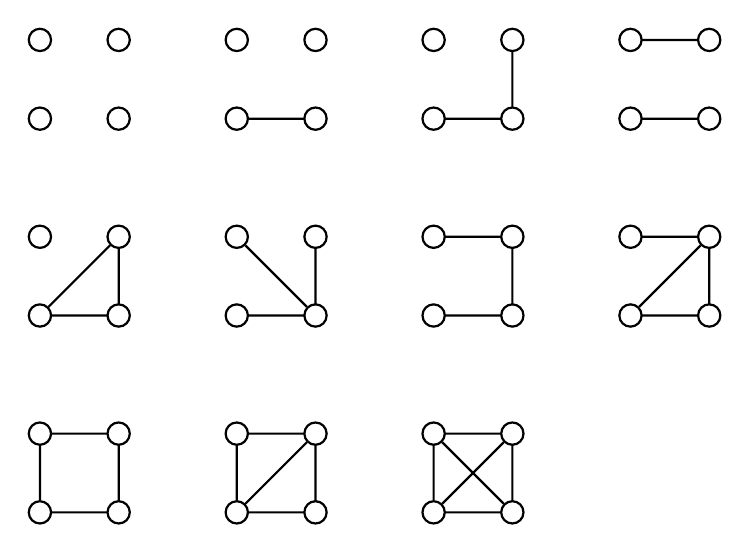
\begin{tikzpicture}[style=thick, scale=0.5]
	\draw
	 (0,0) node (n1) [] {} --
		  ++(2,0) node [] {} --
		  ++(0,2) node [] {} --
		  ++(-2,0) node [] {} -- (n1)
	(5,0) node (n2) [] {} --
		  ++(2,0) node [] {} --
		  ++(0,2) node [] (n21) {} --
		  ++(-2,0) node [] {} -- (n2) -- (n21)
	(10,0) node (n31) [] {} --
		  ++(2,0) node (n32) [] {} --
		  ++(0,2) node (n33) [] {} --
		  ++(-2,0) node (n34) [] {} -- (n31) (n32) -- (n34) (n31) -- (n33)
	(0,5) node (n4) [] {} --
		  ++(2,0) node [] {} --
		  ++(0,2) node (n41) [] {}
		  ++(-2,0) node [] {}
		  (n4) -- (n41)
	(5,5) node (n5) [] {} --
		  ++(2,0) node (n51) [] {} --
		  ++(0,2) node [] {}
		  ++(-2,0) node (n52) [] {}
		  (n51) -- (n52)
	(10,5) node (n6) [] {} --
		  ++(2,0) node (n61) [] {} --
		  ++(0,2) node [] {} --
		  ++(-2,0) node (n62) [] {}
	(15,5) node (n7) [] {} --
		  ++(2,0) node [] {} --
		  ++(0,2) node (n71) [] {} --
		  ++(-2,0) node [] {}
		  (n7) -- (n71)
	(0,10) node (n8) [] {}
		  ++(2,0) node [] {}
		  ++(0,2) node [] {}
		  ++(-2,0) node [] {}
	(5,10) node (n9) [] {} --
		  ++(2,0) node [] {}
		  ++(0,2) node [] {}
		  ++(-2,0) node [] {}
	(10,10) node (n10) [] {} --
		  ++(2,0) node [] {} --
		  ++(0,2) node [] {}
		  ++(-2,0) node [] {}
	(15,10) node (n11) [] {} --
		  ++(2,0) node [] {}
		  ++(0,2) node [] {} --
		  ++(-2,0) node [] {};
\end{tikzpicture}
\end{center}
\caption{Graphs on 4 vertices.}
\label{fig:graphs4}
\end{figure}

Two graphs are isomorphic if there exists a permutation of vertices of
the first graph which produces the second graph.

We think of a graph $G$ on $n$ vertices as a coloring of the edges of
the complete graph $K_n$ with two colors black and white. The black
edges of $K_n$ are present in the graph $G$ and the white are not. Two
graphs $G$ and $H$ on $n$ vertices are isomorphic if there exists an
automorphism of the graph $K_n$ which changes the coloring of $K_n$
corresponding to $G$ to the coloring corresponding to $H$.  The group
of automorphisms of $K_n$ is the symmetric group $S_n$. We need to
compute the action of $S_n$ on the edges of $K_n$ which are the
2-subsets of the set $\{1,2,\ldots,n\}$. We are now ready to compute a
graphs generating function. Let $n=4$.

\begin{example}
(%i1) load(discrete)$
(%i2) grp_v: symmetric_group(4)$
(%i3) grp_e: group_action(grp_v, powerset({1,2,3,4}, 2))$
(%i4) ci: cycle_index_group(grp_e);
(%o4) (6*x[2]*x[4]+8*x[3]^2+9*x[1]^2*x[2]^2+x[1]^6)/24
(%i5) subst_inventory(2, ci);
(%o5) 11
(%i6) subst_inventory([1,t], ci);
(%o6) t^6+t^5+2*t^4+3*t^3+2*t^2+t+1
\end{example}
%
The list of graphs on 4 vertices is shown in Figure \ref{fig:graphs4}.
The coefficient at $t^m$ in the output \verb|%o6|
gives the number of graphs with $m$ edges on four vertices.

%%%%%%%%%%%%%%%%%%%%%%%%%%%%%%%%%%%%%%%%%%%%%%%%%%
%%%%%%%%%%%%%%%%%%%%%%%%%%%%%%%%%%%%%%%%%%%%%%%%%%
%%%%%%%%%%%%%%%%%%%%%%%%%%%%%%%%%%%%%%%%%%%%%%%%%%
\section{Combinatorial species}

The package \command{Species} has functions for counting, listing and
random selection from combinatorial species. Informally, a
combinatorial species is a class of objects which are either atomic or
are constructed with a production rule from other combinatorial
species. A species is labeled, if atoms of size one are labeled with
integers from 1 up to $n$ and unlabeled if atoms are not labeled.

Atomic objects can be atoms which have size 1 or epsilon objects which
have size 0. Productions rules implemented are disjoint union
(\command{Sum}), Cartesian product (\command{Prod}), sequence
(\command{Seq} or \command{Sequence}), sets with repetition
(\command{Multiset} or \command{MSet}), sets without repetition
(\command{Set}) and cycles (\command{Cycle}). Multisets only appear in
unlabeled species.

A \DEF{specification} for combinatorial species is a list of
production rules. We assume that all symbols which appear in a
specification and do not have production rules are atoms.

For example, the specification
$$
\{S=Prod(X, Y), X=Sum(a, b, c), Y=Sum(e, f)\}
$$
defines three combinatorial species. The elements $a, b, c, e, f$ are
atoms, species $X$ contains elements $a, b$ and $c$, species $Y$
contains elements $e$ and $f$ and finally species $S$ contains
$PROD(a, e)$, $PROD(a, f)$, $PROD(b, e)$, $PROD(b, f)$, $PROD(c, e)$,
$PROD(c, f)$.

The \DEF{size} of an element $e$ from a combinatorial species is the
sum of sizes of all atomic objects which appear in $e$. For production
rules \command{Seq}, \command{Set}, \command{MSet} and \command{Cycle}
we also define the \DEF{cardinality}, which is the number of elements
in the sequence, set, multiset and cycle.

For example in specification $\{A=Sum(x, Prod(x,x)), B=Seq(A)\}$ we
have a species $A$ with elements $x$ and $(x,x)$ and a species $B$ of
sequences of elements of $A$. The element $SEQ(x, x, x, PROD(x,x), x,
PROD(x,x))$ has cardinality 6 and size 8.

There is also a special species production rule called \command{Function}.
The rule accepts one arguments which is a function which returns the
number of elements of given size.

%%%%%%%%%%%%%%%%%%%%%%%%%%%%%%%%%%%%%%%%%%%%%%%%%%
%%%%%%%%%%%%%%%%%%%%%%%%%%%%%%%%%%%%%%%%%%%%%%%%%%
\subsection{Counting, listing, random generation}

The main functions in the \command{Species} package are
\command{count\_species}, \command{list\_species} and
\command{select\_from\_species}. All take three arguments: the species
$A$, specification $spec$ and the size $n$.  \command{count\_species}
returns the number of elements of the species $S$ defined by $spec$ of
size $n$, \command{list\_species} returns a list of all elements of
the species $S$ of size $n$ and \command{select\_from\_species}
returns a random element from the species $S$.

Random generation is uniform, if the number of elements of size $n$ is
$a_n$, then the probability that a specific element will be generated
is $\frac{1}{a_n}$.

All three functions will remember all partial results computed which
can be used in later computations. In some situations this memory
needs to be cleared. The memory can be cleared with the function
\command{reset\_species\_memory}.

There is also a function \command{nice\_disp} changes elements
obtained from production rules into lists.

\begin{example}
(%i1) load(Species)$
(%i2) count_species(S, spec, 2);
(%o2) 6
(%i3) list_species(S, spec, 2);
(%o3) [PROD(a,e),PROD(a,f),PROD(b,e),PROD(b,f),
       PROD(c,e),PROD(c,f)]
(%i4) select_from_species(S, spec, 2);
(%o4) PROD(a,e)
(%i5) nice_disp(%);
(%o5) [a,e]
\end{example}

%%%%%%%%%%%%%%%%%%%%%%%%%%%%%%%%%%%%%%%%%%%%%%%%%%
%%%%%%%%%%%%%%%%%%%%%%%%%%%%%%%%%%%%%%%%%%%%%%%%%%
\subsection{Generating functions}

For a combinatorial species $A$ we define its generating function
$A(t)$ as a formal power series
$$
A(t)=\sum_{n=0}^\infty a_nt^n
$$
where $a_n$ is the number of elements of size $n$ in the species $A$.

The function \command{gf\_equations(spec,t)} returns a system of
equations which define the generating functions of species defined by
\command{spec}. If the system is nice the function \command{gf\_solve}
can then be used to compute the generating functions from equations,
or the function \command{gf\_express} can be used to find an equation
for a specific generating function.

\begin{example}
(%i6) spec: [S=Seq(Sum(x, Prod(x,x)))];
(%o6) [S = Seq(Sum(x,Prod(x,x)))]
(%i7) gf_eqs: gf_equations(spec, t);
(%o7) [S(t) = g4323(t)+1,g4323(t) = g4322(t)*S(t),
       g4322(t) = x(t)+g4321(t),g4321(t) = x(t)^2,
       Epsilon(t) = 1,x(t) = t]
(%i8) alg_eq: gf_express(gf_eqs, S(t));
(%o8) (-t^2-t+1)*S(t)-1
(%i9) gf_solve(gf_eqs);
(%o9) [[S(t) = -1/(t^2+t-1),g4323(t) = -(t^2+t)/(t^2+t-1),
        g4322(t) = t^2+t,g4321(t) = t^2,Epsilon(t) = 1,
        x(t) = t]]
\end{example}
%
When the equation for the generating function $A(t)=\sum_{n=0}^\infty
a_nt^n$ is algebraic the function \command{algeq\_to\_rec} (based on
the MuPAD--Combinat function \command{algeqtorec}) can be used to
compute a recurrence relation for the sequence $a_n$. This can be used
to define a function for fast species counting.

\begin{example}
(%i10) rec: algeq_to_rec(alg_eq, S(t));
(%o10) y[n]-y[n-1]-y[n-2]
(%i11) init: makelist(count_species(S, spec, i), i, 1, 2);
(%o11) [1,2]
(%i12) rec_to_function(rec, y[n], init);
(%o12) y_rf[n]:=if n <= 2 then part([1,2],n)
                else y_rf[n-1]+y_rf[n-2]
(%i13) y_rf[30];
(%o13) 1346269
\end{example}

%%%%%%%%%%%%%%%%%%%%%%%%%%%%%%%%%%%%%%%%%%%%%%%%%%
%%%%%%%%%%%%%%%%%%%%%%%%%%%%%%%%%%%%%%%%%%%%%%%%%%
\subsection{Examples}

%%%%%%%%%%%%%%%%%%%%%%%%%%%%%%%%%%%%%%%%%%%%%%%%%%
\subsubsection{Necklaces}

The number necklaces on four vertices with two colors can be computed
with the Cycle production rule.

\begin{example}
(%i1) load(Species)$
(%i2) spec:[N=Cycle(Sum(w,b))];
(%o2) [N = Cycle(Sum(w,b))]
(%i3) count_species(N, spec, 4);
(%o3) 6
(%i4) list_species(N, spec, 4);
(%o4) [CYCLE(w,w,w,w),CYCLE(b,w,w,w),CYCLE(b,w,b,w),
       CYCLE(b,b,w,w),CYCLE(b,b,b,w),CYCLE(b,b,b,b)]
\end{example}
%
Compare this with the necklace example in the P\'olya theory section.

\subsubsection{Trees}

A \DEF{rooted binary tree} can be defined as a leaf or an internal
node with two binary subtrees (see Figure \ref{fig:btdef}). Binary
trees with $n$ leaves can be counted with the following specification

\begin{figure}
\begin{center}
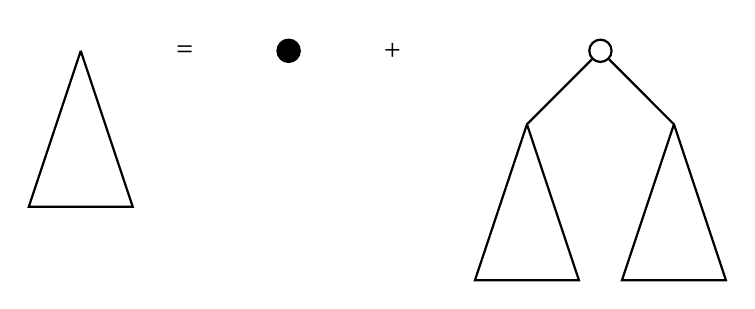
\begin{tikzpicture}[style=thick,scale=0.66]
\draw (0,5) -- ++ (-1,-3) -- ++ (2, 0) -- ++ (-1, 3)
	(2,5) node [draw=white] {=}
	(4,5) node [fill=black] {}
	(6,5) node [draw=white] {+}
	(10,5) node (r) [] {}
	(r) -- ++ (-45:2) -- ++ (-1,-3) -- ++ (2, 0) -- ++ (-1, 3)
	(r) -- ++ (225:2) -- ++ (-1,-3) -- ++ (2, 0) -- ++ (-1, 3);
\end{tikzpicture}
\end{center}
\caption{Decomposition of a binary tree into smaller binary trees.}
\label{fig:btdef}
\end{figure}

\begin{example}
(%i1) load(Species)$
(%i2) spec: [T=Sum(x, Prod(T, T))];
(%o2) [T = Sum(x,Prod(T,T))]
(%i3) makelist(count_species(T, spec, i), i, 1, 10);
(%o3) [1,1,2,5,14,42,132,429,1430,4862]
\end{example}
%
The generating functions can be used to efficiently count
the binary trees for large number of leaves.

\begin{example}
(%i4) gf_equations(spec, t);
(%o4) [T(t) = x(t)+g4255(t),g4255(t) = T(t)^2,x(t) = t]
(%i5) gf_express(%, T(t));
(%o5) T(t)^2-T(t)+t
(%i6) algeq_to_rec(%, T(t));
(%o6) n*y[n]+(6-4*n)*y[n-1]
(%i7) rec_to_function(%, y[n], [1,1])$
(%i8) y_rf[100];
(%o8) 227508830794229349661819540395688853956041682601541047340
(%i9) nice_disp(select_from_species(T, spec, 5));
(%o9) [x,[x,[[x,x],x]]]
\end{example}
%
The random selection corresponds to the tree in Figure \ref{fig:tree}.

\begin{figure}
\begin{center}
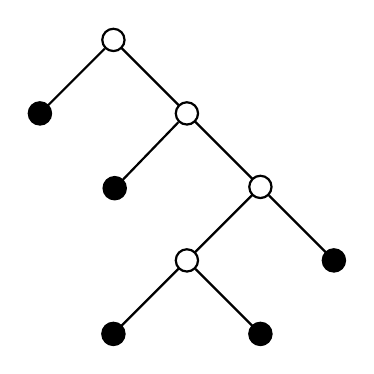
\begin{tikzpicture}[style=thick, scale=0.66]
	\draw (0,0) node (n1) [] {} --
	++(-45:2) node (n2) [] {} --
	++ (-45:2) node (n3) [] {} --
	++ (-135:2) node (n4) [] {} --
	++ (-135:2) node (n5) [fill=black] {}
	(n4) -- ++ (-45:2) node (n6) [fill=black] {}
	(n3) -- ++ (-45:2) node (n7) [fill=black] {}
	(n2) -- ++ (-134:2) node (n8) [fill=black] {}
	(n1) -- ++ (-135:2) node (n9) [fill=black] {};
\end{tikzpicture}
\end{center}
\caption{A random binary tree with 5 leaves.}
\label{fig:tree}
\end{figure}

A \DEF{ternary tree} is a rooted tree in which each node has at most
three children. We do not distinguish between two trees if one can be
obtained from the other by permuting the children of some nodes.

Ternary trees can be counted with the following specification.

\begin{example}
(%i10) spec: [TT=Prod(x, MSet(TT, max_card=3))]$
(%i11) makelist(count_species(TT, spec, i), i, 1, 15);
(%o11) [1,1,2,4,8,17,39,89,211,507,1238,3057,7639,19241,48865]
\end{example}
%
The function \command{tree\_disp} nicely prints a tree.
\begin{example}
(%i12) tree_disp(tree) := tree_disp1(tree, 1)$
       tree_disp1(tree, d) := (
         if length(tree)>0 then
           printf(true,"~{~a~}\\-- ~a~%",makelist(" ",d),first(tree)),
         if length(tree)>1 then
           map(lambda([t],tree_disp1(t,d+4)),second(tree)))$
\end{example}
%
A random ternary tree on 12 nodes (Figure \ref{fig:tt}) nicely
printed with the \command{tree\_disp} function.
\begin{example}
(%i13) tree: nice_disp(select_from_species(TT, spec, 12))$
(%i14) tree_disp(tree)$
 \-- x
     \-- x
         \-- x
         \-- x
     \-- x
         \-- x
         \-- x
         \-- x
     \-- x
         \-- x
             \-- x
             \-- x
\end{example}

\begin{figure}
\begin{center}
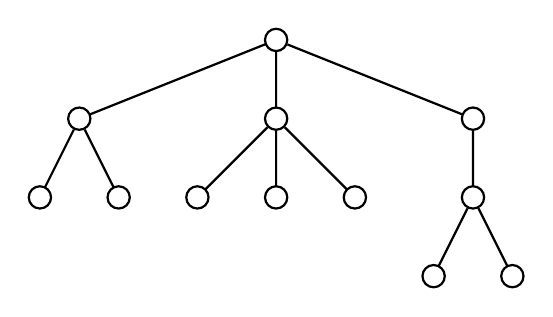
\begin{tikzpicture}[style=thick, scale=0.5]
	\draw (0,0) node (n1) {} --
		++ (-5, -2) node (n2) {}
		(n2) -- ++(-1,-2) node () {}
		(n2) -- ++ (1,-2) node () {}
		(n1) -- ++(0, -2) node (n3) {}
		(n3) -- ++(-2,-2) node () {}
		(n3) -- ++(0,-2) node () {}
		(n3) -- ++(2,-2) node () {}
		(n1) -- ++(5,-2) node () {} -- ++(0,-2) node (n4) {}
		(n4) -- ++(-1,-2) node () {}
		(n4) -- ++(1,-2) node () {};
\end{tikzpicture}
\end{center}
\caption{A random ternary tree.}
\label{fig:tt}
\end{figure}

%%%%%%%%%%%%%%%%%%%%%%%%%%%%%%%%%%%%%%%%%%%%%%%%%%
\subsubsection{Monotonic paths}

A monotonic path is a path along the edges of a $n\times n$ grid which
starts at $(0,0)$, ends at $(n,n)$ and is always above the diagonal.
Monotonic paths can be counted with the following specification.

\begin{figure}
\begin{center}
\begin{tikzpicture}[style=thick, scale=0.75]
	\draw [->, decorate, decoration=snake] (0,3) -- (2,5);
	\draw (3,5) node [draw=white] {=};
	\draw (4,5) node [draw=white] {$\epsilon$};
	\draw (5,5) node [draw=white] {+};
	\draw[ultra thick, ->] (6,0) -- (6,1);
	\draw [->, decorate, decoration=snake] (6,1) -- (8,3);
	\draw[ultra thick, ->] (8,3) -- (9,3);
	\draw [->, decorate, decoration=snake] (9,3) -- (11,5);
\end{tikzpicture}
\end{center}
\caption{Decomposition of a monotonic path into smaller monotonic paths.}
\label{fig:MPspec}
\end{figure}

\begin{example}
(%i1) load(Species)$
(%i2) spec: [MP=Sum(Epsilon, Prod(Up, MP, Right, MP)),
             Right=Epsilon]$
(%i3) makelist(count_species(MP, spec, i),i,1,10);
(%o3) [1,2,5,14,42,132,429,1430,4862,16796]
\end{example}
%
The sequence is similar to number of binary trees. The numbers in the
sequence are known as Catalan numbers $C_n=\frac{1}{n+1}{2n \choose n}$.

\begin{figure}
\begin{center}
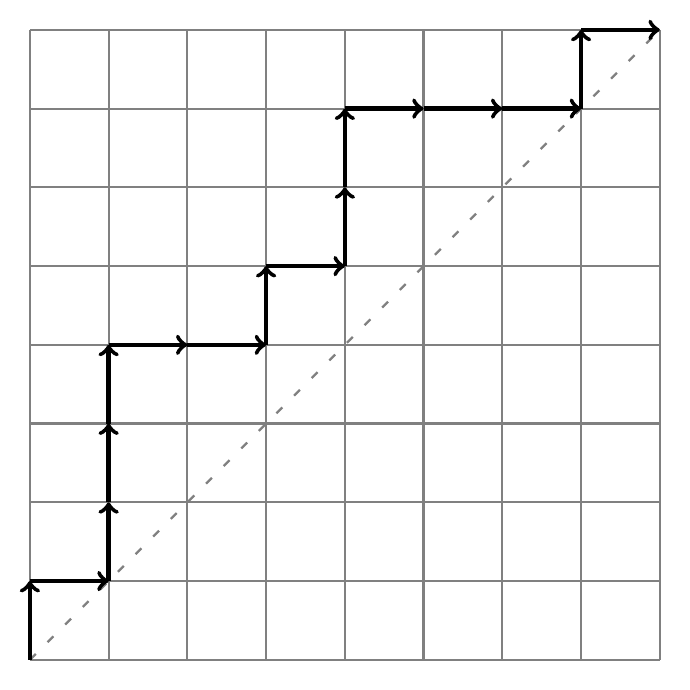
\begin{tikzpicture}[style=thick, scale=0.5]
	\draw[gray, step=2] (0,0) grid (16,16);
	\draw[gray, loosely dashed] (0,0) -- (16,16);
	\draw[->, ultra thick] (0,0) -- (0,2);
	\draw[->, ultra thick] (0,2) -- (2,2);
	\draw[->, ultra thick] (2,2) -- (2,4);
	\draw[->, ultra thick] (2,4) -- (2,6);
	\draw[->, ultra thick] (2,6) -- (2,8);
	\draw[->, ultra thick] (2,8) -- (4,8);
	\draw[->, ultra thick] (4,8) -- (6,8);
	\draw[->, ultra thick] (6,8) -- (6,10);
	\draw[->, ultra thick] (6,10) -- (8,10);
	\draw[->, ultra thick] (8,10) -- (8,12);
	\draw[->, ultra thick] (8,12) -- (8,14);
	\draw[->, ultra thick] (8,14) -- (10,14);
	\draw[->, ultra thick] (10,14) -- (12,14);
	\draw[->, ultra thick] (12,14) -- (14,14);
	\draw[->, ultra thick] (14,14) -- (14,16);
	\draw[->, ultra thick] (14,16) -- (16,16);
\end{tikzpicture}
\end{center}
\caption{A random monotonic path.}
\label{fig:MP}
\end{figure}

\begin{example}
(%i4) makelist(binomial(2*n,n)/(n+1),n,1,10);
(%o4) [1,2,5,14,42,132,429,1430,4862,16796]
\end{example}
%
A random monotonic path of length 8 is shown in Figure \ref{fig:MP}.

\begin{example}
(%i5) flatten(nice_disp1(select_from_species(MP, spec, 8)));
(%o5) [Up,Right,Up,Up,Up,Right,Right,Up,Right,Up,Up,Right,Right,
       Right,Up,Right]
\end{example}
%
We can find the explicit formula for the number of monotonic paths of
length $n$ from the generating functions.

\begin{example}
(%i6) gf_equations(spec, t)$
(%i7) gf_express(%, MP(t));
(%o7) t*MP(t)^2-MP(t)+1
(%i8) algeq_to_rec(%, MP(t));
(%o8) (n+1)*y[n]+(2-4*n)*y[n-1]
(%i9) solve_rec(%, y[n], y[1]=1);
(%o9) y[n] = 2^(2*n)*gamma(n+1/2)/(sqrt(%pi)*(n+1)!)
\end{example}

%%%%%%%%%%%%%%%%%%%%%%%%%%%%%%%%%%%%%%%%%%%%%%%%%%
\subsubsection{Integer partitions}

We will use the \command{Function} production rule to define a species
of (subset of) integers. We assume that the size of an integer $n$ is
$n$.  An integer partition of $n$ is then a multiset of integers of
size $n$.

\begin{example}
(%i1) load(Species)$
(%i2) cnt_ints(n) := if n>0 then 1 else 0$
(%i3) specIP: [IP=MSet(N), N=Function(cnt_ints)]$
(%i4) count_species(IP, specIP, 100);
(%o4) 190569292
(%i5) num_partitions(100);
(%o5) 190569292
(%i6) nice_disp(select_from_species(IP, specIP, 100));
(%o6) [1,1,1,1,1,1,1,1,3,3,3,3,3,3,3,3,7,7,7,15,32]
\end{example}
%
Of course the counting function can be more complicated. In the
following example we count the number of partitions of 100 into two
primes and two squares.

\begin{example}
(%i7) cnt_primes(n) := if primep(n) then 1 else 0$
(%i8) cnt_squares(n) := if integerp(sqrt(n)) then 1 else 0$
(%i9) specIP: [IP=Prod(P, P, S, S),
                P=Function(cnt_primes),
                S=Function(cnt_squares)]$
(%i10) count_species(IP, specIP, 100);
(%o10) 397
(%i11) flatten(nice_disp(select_from_species(IP, specIP, 100)));
(%o11) [13,67,4,16]
\end{example}
%
We can also count the number of partitions of an integer $n$ into
three primes.

\begin{example}
(%i12) specIPP: [IP=MSet(P, card=3), P=Function(cnt_primes)]$
(%i13) makelist(count_species(IP, specIPP, i), i, 6, 100);
(%o13) [1,1,1,2,1,2,2,2,1,3,2,4,2,3,2,5,2,5,3,5,3,7,3,7,2,6,3,9,2,8,
        4,9,4,10,2,11,3,10,4,12,3,13,4,12,5,15,4,16,3,14,5,17,3,16,4,
        16,6,19,3,21,5,20,6,20,2,22,5,21,6,22,5,28,5,24,7,25,4,29,5,
        27,8,29,5,33,4,29,9,33,4,35,5,34,7,30,3]
(%i14) nice_disp(select_from_species(IP, specIPP, 301));
(%o14) [13,47,241]
\end{example}

%%%%%%%%%%%%%%%%%%%%%%%%%%%%%%%%%%%%%%%%%%%%%%%%%%
\subsubsection{Sequences}

A sequence $a_1a_2a_3a_4\cdots$ can be represented as $Prod(a_1,
Prod(a_2, Prod(a_3, \cdots )))$. This enables us to count sequences
with special properties.

In the next example we investigate the number of words of length $n$
with letters a, b and c in which each letter appears an even number of
times. We define species $AeBeCe$, $AeBeCo$, $\ldots$ which represent
words in which each letter appears an even number of times; a, b
appear an even number of times and c an odd number of times $\ldots$

\begin{example}
(%i1) load(Species)$
(%i2) spec:[
        AeBeCe=Sum(Epsilon,
                   Prod(A,AoBeCe), Prod(B,AeBoCe), Prod(C,AeBeCo)),
        AeBeCo=Sum(Prod(A,AoBeCo), Prod(B,AeBoCo), Prod(C,AeBeCe)),
        AeBoCe=Sum(Prod(A,AoBoCe), Prod(B,AeBeCe), Prod(C,AeBoCo)),
        AeBoCo=Sum(Prod(A,AoBoCo), Prod(B,AeBeCo), Prod(C,AeBoCe)),
        AoBeCe=Sum(Prod(A,AeBeCe), Prod(B,AoBoCe), Prod(C,AoBeCo)),
        AoBeCo=Sum(Prod(A,AeBeCo), Prod(B,AoBoCo), Prod(C,AoBeCe)),
        AoBoCe=Sum(Prod(A,AeBoCe), Prod(B,AoBeCe), Prod(C,AoBoCo)),
        AoBoCo=Sum(Prod(A,AeBoCo), Prod(B,AoBeCo), Prod(C,AoBoCe))
      ]$
(%i3) makelist(count_species(AeBeCe, spec, i), i, 0, 20);
(%o3) [1,0,3,0,21,0,183,0,1641,0,14763,0,132861,0,1195743,
       0,10761681,0,96855123,0,871696101]
(%i4) makelist(count_species(AeBoCo, spec, i), i, 0, 20);
(%o4) [0,0,2,0,20,0,182,0,1640,0,14762,0,132860,0,1195742,
       0,10761680,0,96855122,0,871696100]
(%i5) makelist(count_species(AoBoCo, spec, i), i, 0, 20);
(%o5) [0,0,0,6,0,60,0,546,0,4920,0,44286,0,398580,0,
       3587226,0,32285040,0,290565366,0]
(%i6) makelist(count_species(AoBeCe, spec, i), i, 0, 20);
(%o6) [0,1,0,7,0,61,0,547,0,4921,0,44287,0,398581,0,
       3587227,0,32285041,0,290565367,0]
\end{example}
%
We see that for odd $n$ there are no sequences in $AeBeCe$ and for
even $n$ there is one more sequence in $AeBeCe$ than in $AeBoCo$. We
can further investigate the generating functions.

\begin{example}
(%i7) eqns: gf_equations(spec, t)$
(%i8) eqns_sol: gf_solve(eqns)$
(%i9) AeBeCe_gf: assoc(AeBeCe(t), first(eqns_sol));
(%o9) -(7*t^2-1)/(9*t^4-10*t^2+1)
(%i10) AeBeCe_rec: ratfun_to_rec(AeBeCe_gf);
(%o10) -y[n]+10*y[n-2]-9*y[n-4]
(%i11) AeBeCe_sol: solve_rec(AeBeCe_rec, y[n],
         y[0]=1, y[1]=0, y[2]=3, y[3]=0);
(%o11) y[n] = 3^n/8+3*(-1)^n/8+(-3)^n/8+3/8
(%i12) declare(n, integer)$
(%i13) subst(n=2*n,AeBeCe_sol);
(%o13) y[2*n] = 3^(2*n)/4+3/4
\end{example}

%%%%%%%%%%%%%%%%%%%%%%%%%%%%%%%%%%%%%%%%%%%%%%%%%%
\subsubsection{Building towers}

\begin{figure}[p]
\begin{center}
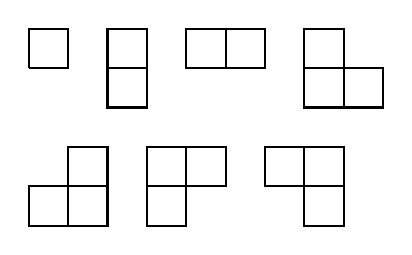
\begin{tikzpicture}[style=thick, scale=0.5]
	\draw (2,1) -- (0,1) -- (0,0) -- (2,0) -- (2,2) -- (1,2) -- (1,0);
	\draw (3,1) -- (5,1) -- (5,2) -- (3,2) -- (3,0) -- (4,0) -- (4,2);
	\draw (7,2) -- (7,0) -- (8,0) -- (8,2) -- (6,2) -- (6,1) -- (8,1);
	\draw (0,4) -- (1,4) -- (1,5) -- (0,5) -- (0,4);
	\draw (2,4) -- (3,4) -- (3,5) -- (2,5) -- (2,3) -- (3,3) -- (3,4);
	\draw (5,5) -- (5,4) -- (6,4) -- (6,5) -- (4,5) -- (4,4) -- (5,4);
	\draw (8,3) -- (8,5) -- (7,5) -- (7,3) -- (9,3) -- (9,4) -- (7,4);
\end{tikzpicture}
\end{center}
\caption{Blocks used for building towers.}
\label{fig:blocks}
\end{figure}

\begin{figure}[p]
\begin{center}
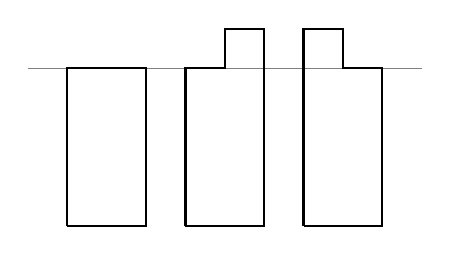
\begin{tikzpicture}[style=thick, scale=0.5]
	\draw [very thin, gray] (-1,4) -- (9,4);
	\draw
		(0,0) -- (2,0) -- (2,4) -- (0,4) -- (0,0)
		(3,0) -- (5,0) -- (5,5) -- (4,5) -- (4,4) -- (3,4) -- (3,0)
		(6,0) -- (8,0) -- (8,4) -- (7,4) -- (7,5) -- (6,5) -- (6,0);
\end{tikzpicture}
\end{center}
\caption{Towers species of size $n$.}
\label{fig:towers}
\end{figure}

\begin{figure}[p]
\begin{center}
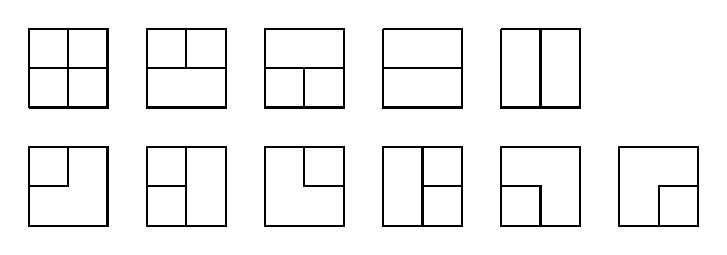
\begin{tikzpicture}[style=thick, scale=0.5]
	\draw (0,3) -- (2,3) -- (2,5) -- (0,5) -- (0,3);
		\draw (0,4) -- (2,4);
		\draw (1,3) -- (1,5);
	\draw (3,4) -- (5,4) -- (5,3) -- (3,3) -- (3,5) -- (5,5) -- (5,4);
		\draw (4,5) -- (4,4);
	\draw (6,4) -- (8,4) -- (8,3) -- (6,3) -- (6,5) -- (8,5) -- (8,4);
		\draw (7,4) -- (7,3);
	\draw (9,5) -- (11,5) -- (11,3) -- (9,3) -- (9,5);
		\draw (9,4) -- (11,4);
	\draw (12,5) -- (14,5) -- (14,3) -- (12,3) -- (12,5);
		\draw (13,3) -- (13,5);
	\draw (0,1) -- (1,1) -- (1,2) -- (0,2) -- (0,0) -- (2,0) --
		 (2,2) -- (1,2);
	\draw (4,0) -- (4,2) -- (3,2) -- (3,0) -- (5,0) -- (5,2) -- (4,2);
		\draw (3,1) -- (4,1);
	\draw (7,2) -- (7,1) -- (8,1) -- (8,2) -- (6,2) -- (6,0) --
		(8,0) -- (8,2);
	\draw (10,2) -- (10,0) -- (11,0) -- (11,2) -- (9,2) --
		(9,0) -- (10,0);
		\draw (10,1) -- (11,1);
	\draw (12,1) -- (13,1) -- (13,0) -- (14,0) -- (14,2) --
		(12,2) -- (12,0) -- (13,0);
	\draw (17,1) -- (16,1) -- (16,0) -- (17,0) -- (17,2) --
		(15,2) -- (15,0) -- (16,0);
\end{tikzpicture}
\end{center}
\caption{Towers of size 2.}
\label{fig:towers2}
\end{figure}

\begin{figure}[p]
\begin{center}
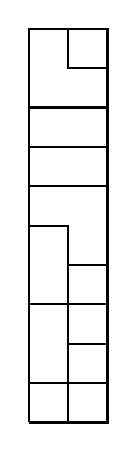
\begin{tikzpicture}[style=thick, scale=0.5]
	\draw (0,0) -- (2,0) -- (2,10) -- (0,10) -- (0,0);
	\draw (1,0) -- (1,4) -- (2,4);
	\draw (0,3) -- (2,3);
	\draw (1,2) -- (2,2);
	\draw (0,1) -- (2,1);
	\draw (1,4) -- (1,5) -- (0,5);
	\draw (0,6) -- (2,6);
	\draw (0,7) -- (2,7);
	\draw (0,8) -- (2,8);
	\draw (1,10) -- (1,9) -- (2,9);
\end{tikzpicture}
\end{center}
\caption{A random tower of size 10.}
\label{fig:tower10}
\end{figure}

We count the number of different ways to build a two column tower with
blocks shown in Figure \ref{fig:blocks}. We name the block with
letters S, V, H, L1, L2, L3 and L4 from left to right, up to
bottom. For blocks S and V we add the number of the column in which
the block sits.

If we draw a line at the height $n$ we will have three possibilities
(Figure \ref{fig:towers}). The line does not intersect any block
(species $LL$), it intersects a block V or L2 in the second column and
no block in the first column (species $LP$) or it intersects a block V
or L1 in the first column and no block in the second column (species
$PL$). Note that if the line intersects L3 in the first column and no
block in the second column this belongs to the species LL of size
$n+1$. In the specification there is a symbol \command{x} for the size
of the tower. We also have symbols for blocks which are of size 0.
Here is a specification for the species.

\begin{example}
(%i1) load(Species)$
(%i2) spec: [
        LL=Sum(Epsilon,
          Prod(x, LL, S1, S2),
          Prod(x, LL, H),
          Prod(x,x, LL, V1, V2),
          Prod(x, LP, S1),
          Prod(x, PL, S2),
          Prod(x,x, LP, L3),
          Prod(x,x, LL, S1, L4),
          Prod(x,x, LL, L3, S2),
          Prod(x,x, PL, L4)),
        LP=Sum(
          Prod(x, LL, L2),
          Prod(x, PL, V2),
          Prod(x, LL, S1, V2)),
        PL=Sum(
          Prod(x, LL, L1),
          Prod(x, LP, V1),
          Prod(x, LL, V1, S2)),
        S1=Epsilon, S2=Epsilon, V1=Epsilon, V2=Epsilon, H=Epsilon,
        L1=Epsilon, L2=Epsilon, L3=Epsilon, L4=Epsilon]$
\end{example}
%
We can list the towers of size 2 (shown in Figure \ref{fig:towers2}).

\begin{example}
(%i3) list_species(LL, spec, 2)$
(%i4) map(lambda([f], rest(flatten(f), 3)), nice_disp(%));
(%o4) [[S1,S2,S1,S2],[H,S1,S2],[S1,S2,H],[H,H],[V1,V2],
       [L2,S1],[S1,V2,S1],[L1,S2],[V1,S2,S2],[S1,L4],
       [L3,S2]]
\end{example}
%
Or choose a random tower of size 10 (shown in Figure \ref{fig:tower10}).
\begin{example}
(%i5) select_from_species(LL, spec, 10)$
(%i6) rest(flatten(nice_disp(%)), 11);
(%o6) [S1,S2,V1,S2,S2,V1,S2,L4,H,H,L1,S2]
\end{example}
%
Using the generating functions we can find an explicit formula for
the number of towers of size $n$. Since the system is complicated
we use Gr\"obner bases to express $LL(t)$.

\begin{example}
(%i7) makelist(count_species(LL, spec, i), i, 0, 5);
(%o7) [1,2,11,44,189,798]
(%i8) eqs: gf_equations(spec, t)$
(%i9) LL_eq: gf_express(eqs, LL(t), use_grobner=true);
(%o9) (-t^3-5*t^2-3*t+1)*LL(t)+t-1
(%i10) LL_rec: algeq_to_rec(LL_eq, LL(t));
(%o10) y[n]-3*y[n-1]-5*y[n-2]-y[n-3]
(%i11) LL_explicit: solve_rec(LL_rec,y[n],y[0]=1,y[1]=2,y[2]=11);
(%o11) y[n] = (-1)^n/2+(sqrt(5)+2)^n*(3*sqrt(5)+5)/20
                      -(2-sqrt(5))^n*(3*sqrt(5)-5)/20
\end{example}
which is
$$
{y}_{n}=\frac{{\left( -1\right) }^{n}}{2}+\frac{{\left( \sqrt{5}+2\right) }^{n}\,\left( 3\,\sqrt{5}+5\right) }{20}-\frac{{\left( 2-\sqrt{5}\right) }^{n}\,\left( 3\,\sqrt{5}-5\right) }{20}.
$$

\begin{thebibliography}{10}

\bibitem{Max} Maxima computer algebra system,
	\LINK{http://maxima.sourceforge.net/}
\bibitem{P} P\'olya, G., {\em Kombinatorische Anzahlbestimmungen
	f\"ur Gruppen, Graphen und chemische Verbindungen},
	Acta Math. 68 (1937), 145--254.
\bibitem{J} Joyal, A., {\em Une th\'eorie combinatoire des
	s\'eries formelles}, Advances in Mathematics 42, 1 (1981), 1--82.
\bibitem{BLL}  Bergeron F., Labelle G., Leroux P.,
	{\em Combinatorial Species and Tree-Like Structures}
	Encyclopedia of Mathematics and Its Applications 67,
	Cambridge University Press, Cambridge (1998).
\bibitem{AC} Hemmecke R., Rubey M.,
	{\em Aldor--Combinat: An Implementation of Combinatorial Species},\\
	\LINK{http://www.risc.uni-linz.ac.at/people/hemmecke/aldor/combinat/}
\bibitem{MCS} Denise A., Dutour I., Zimmermann P.,
	{\em Cs: a MuPAD package for counting and randomly generating
	combinatorial structures},
	In Proceedings of FPSAC'98, 1998, 195--204.
\bibitem{MC} \LINK{http://mupad-combinat.sourceforge.net/}
\bibitem{sage} \LINK{http://sagemath.org/}
\bibitem{bliss} \LINK{http://www.tcs.hut.fi/Software/bliss/index.html}

\end{thebibliography}

\end{document}

% LocalWords:  Andrej Vodopivec olya combinatorics olya's maxima automorphisms
% LocalWords:  monomial subst
